\documentclass[9pt]{IEEEtran}
\linespread{0.922}

% journal
%
% If IEEEtran.cls has not been installed into the LaTeX system files,
% manually specify the path to it like:
% \documentclass[journal]{../sty/IEEEtran}

% Some very useful LaTeX packages include:
% (uncomment the ones you want to load)

% *** MISC UTILITY PACKAGES ***
%
%\usepackage{ifpdf}
% Heiko Oberdiek's ifpdf.sty is very useful if you need conditional
% compilation based on whether the output is pdf or dvi.
% usage:
% \ifpdf
%   % pdf code
% \else
%   % dvi code
% \fi
% The latest version of ifpdf.sty can be obtained from:
% http://www.ctan.org/pkg/ifpdf
% Also, note that IEEEtran.cls V1.7 and later provides a builtin
% \ifCLASSINFOpdf conditional that works the same way.
% When switching from latex to pdflatex and vice-versa, the compiler may
% have to be run twice to clear warning/error messages.

% *** CITATION PACKAGES ***
%
%\usepackage{cite}
% cite.sty was written by Donald Arseneau
% V1.6 and later of IEEEtran pre-defines the format of the cite.sty package
% \cite{} output to follow that of the IEEE. Loading the cite package will
% result in citation numbers being automatically sorted and properly
% "compressed/ranged". e.g., [1], [9], [2], [7], [5], [6] without using
% cite.sty will become [1], [2], [5]--[7], [9] using cite.sty. cite.sty's
% \cite will automatically add leading space, if needed. Use cite.sty's
% noadjust option (cite.sty V3.8 and later) if you want to turn this off
% such as if a citation ever needs to be enclosed in parenthesis.
% cite.sty is already installed on most LaTeX systems. Be sure and use
% version 5.0 (2009-03-20) and later if using hyperref.sty.
% The latest version can be obtained at:
% http://www.ctan.org/pkg/cite
% The documentation is contained in the cite.sty file itself.

\usepackage[pdftex]{graphicx}
\usepackage{subcaption}

% *** GRAPHICS RELATED PACKAGES ***
%
\ifCLASSINFOpdf
  % \usepackage[pdftex]{graphicx}
  % declare the path(s) where your graphic files are
  % \graphicspath{{../pdf/}{../jpeg/}}
  % and their extensions so you won't have to specify these with
  % every instance of \includegraphics
  % \DeclareGraphicsExtensions{.pdf,.jpeg,.png}
\else
  % or other class option (dvipsone, dvipdf, if not using dvips). graphicx
  % will default to the driver specified in the system graphics.cfg if no
  % driver is specified.
  % \usepackage[dvips]{graphicx}
  % declare the path(s) where your graphic files are
  % \graphicspath{{../eps/}}
  % and their extensions so you won't have to specify these with
  % every instance of \includegraphics
  % \DeclareGraphicsExtensions{.eps}
\fi

% graphicx was written by David Carlisle and Sebastian Rahtz. It is
% required if you want graphics, photos, etc. graphicx.sty is already
% installed on most LaTeX systems. The latest version and documentation
% can be obtained at: 
% http://www.ctan.org/pkg/graphicx
% Another good source of documentation is "Using Imported Graphics in
% LaTeX2e" by Keith Reckdahl which can be found at:
% http://www.ctan.org/pkg/epslatex
%
% latex, and pdflatex in dvi mode, support graphics in encapsulated
% postscript (.eps) format. pdflatex in pdf mode supports graphics
% in .pdf, .jpeg, .png and .mps (metapost) formats. Users should ensure
% that all non-photo figures use a vector format (.eps, .pdf, .mps) and
% not a bitmapped formats (.jpeg, .png). The IEEE frowns on bitmapped formats
% which can result in "jaggedy"/blurry rendering of lines and letters as
% well as large increases in file sizes.
%
% You can find documentation about the pdfTeX application at:
% http://www.tug.org/applications/pdftex

% *** MATH PACKAGES ***
%
\usepackage{amsmath}
% A popular package from the American Mathematical Society that provides
% many useful and powerful commands for dealing with mathematics.
%
% Note that the amsmath package sets \interdisplaylinepenalty to 10000
% thus preventing page breaks from occurring within multiline equations. Use:
%\interdisplaylinepenalty=2500
% after loading amsmath to restore such page breaks as IEEEtran.cls normally
% does. amsmath.sty is already installed on most LaTeX systems. The latest
% version and documentation can be obtained at:
% http://www.ctan.org/pkg/amsmath

\usepackage{bm}
\usepackage{amssymb} %FOR MATHBB

% *** SPECIALIZED LIST PACKAGES ***
%
\usepackage{algorithm}
\usepackage{algorithmic}
% algorithmic.sty was written by Peter Williams and Rogerio Brito.
% This package provides an algorithmic environment fo describing algorithms.
% You can use the algorithmic environment in-text or within a figure
% environment to provide for a floating algorithm. Do NOT use the algorithm
% floating environment provided by algorithm.sty (by the same authors) or
% algorithm2e.sty (by Christophe Fiorio) as the IEEE does not use dedicated
% algorithm float types and packages that provide these will not provide
% correct IEEE style captions. The latest version and documentation of
% algorithmic.sty can be obtained at:
% http://www.ctan.org/pkg/algorithms
% Also of interest may be the (relatively newer and more customizable)
% algorithmicx.sty package by Szasz Janos:
% http://www.ctan.org/pkg/algorithmicx

% *** ALIGNMENT PACKAGES ***
%
%\usepackage{array}
% Frank Mittelbach's and David Carlisle's array.sty patches and improves
% the standard LaTeX2e array and tabular environments to provide better
% appearance and additional user controls. As the default LaTeX2e table
% generation code is lacking to the point of almost being broken with
% respect to the quality of the end results, all users are strongly
% advised to use an enhanced (at the very least that provided by array.sty)
% set of table tools. array.sty is already installed on most systems. The
% latest version and documentation can be obtained at:
% http://www.ctan.org/pkg/array

% IEEEtran contains the IEEEeqnarray family of commands that can be used to
% generate multiline equations as well as matrices, tables, etc., of high
% quality.

% *** SUBFIGURE PACKAGES ***
%\ifCLASSOPTIONcompsoc
%  \usepackage[caption=false,font=normalsize,labelfont=sf,textfont=sf]{subfig}
%\else
%  \usepackage[caption=false,font=footnotesize]{subfig}
%\fi
% subfig.sty, written by Steven Douglas Cochran, is the modern replacement
% for subfigure.sty, the latter of which is no longer maintained and is
% incompatible with some LaTeX packages including fixltx2e. However,
% subfig.sty requires and automatically loads Axel Sommerfeldt's caption.sty
% which will override IEEEtran.cls' handling of captions and this will result
% in non-IEEE style figure/table captions. To prevent this problem, be sure
% and invoke subfig.sty's "caption=false" package option (available since
% subfig.sty version 1.3, 2005/06/28) as this is will preserve IEEEtran.cls
% handling of captions.
% Note that the Computer Society format requires a larger sans serif font
% than the serif footnote size font used in traditional IEEE formatting
% and thus the need to invoke different subfig.sty package options depending
% on whether compsoc mode has been enabled.
%
% The latest version and documentation of subfig.sty can be obtained at:
% http://www.ctan.org/pkg/subfig

% *** FLOAT PACKAGES ***
%
%\usepackage{fixltx2e}
% fixltx2e, the successor to the earlier fix2col.sty, was written by
% Frank Mittelbach and David Carlisle. This package corrects a few problems
% in the LaTeX2e kernel, the most notable of which is that in current
% LaTeX2e releases, the ordering of single and double column floats is not
% guaranteed to be preserved. Thus, an unpatched LaTeX2e can allow a
% single column figure to be placed prior to an earlier double column
% figure.
% Be aware that LaTeX2e kernels dated 2015 and later have fixltx2e.sty's
% corrections already built into the system in which case a warning will
% be issued if an attempt is made to load fixltx2e.sty as it is no longer
% needed.
% The latest version and documentation can be found at:
% http://www.ctan.org/pkg/fixltx2e

%\usepackage{stfloats}
% stfloats.sty was written by Sigitas Tolusis. This package gives LaTeX2e
% the ability to do double column floats at the bottom of the page as well
% as the top. (e.g., "\begin{figure*}[!b]" is not normally possible in
% LaTeX2e). It also provides a command:
%\fnbelowfloat
% to enable the placement of footnotes below bottom floats (the standard
% LaTeX2e kernel puts them above bottom floats). This is an invasive package
% which rewrites many portions of the LaTeX2e float routines. It may not work
% with other packages that modify the LaTeX2e float routines. The latest
% version and documentation can be obtained at:
% http://www.ctan.org/pkg/stfloats
% Do not use the stfloats baselinefloat ability as the IEEE does not allow
% \baselineskip to stretch. Authors submitting work to the IEEE should note
% that the IEEE rarely uses double column equations and that authors should try
% to avoid such use. Do not be tempted to use the cuted.sty or midfloat.sty
% packages (also by Sigitas Tolusis) as the IEEE does not format its papers in
% such ways.
% Do not attempt to use stfloats with fixltx2e as they are incompatible.
% Instead, use Morten Hogholm'a dblfloatfix which combines the features
% of both fixltx2e and stfloats:
%
% \usepackage{dblfloatfix}
% The latest version can be found at:
% http://www.ctan.org/pkg/dblfloatfix

%\ifCLASSOPTIONcaptionsoff
%  \usepackage[nomarkers]{endfloat}
% \let\MYoriglatexcaption\caption
% \renewcommand{\caption}[2][\relax]{\MYoriglatexcaption[#2]{#2}}
%\fi
% endfloat.sty was written by James Darrell McCauley, Jeff Goldberg and 
% Axel Sommerfeldt. This package may be useful when used in conjunction with 
% IEEEtran.cls'  captionsoff option. Some IEEE journals/societies require that
% submissions have lists of figures/tables at the end of the paper and that
% figures/tables without any captions are placed on a page by themselves at
% the end of the document. If needed, the draftcls IEEEtran class option or
% \CLASSINPUTbaselinestretch interface can be used to increase the line
% spacing as well. Be sure and use the nomarkers option of endfloat to
% prevent endfloat from "marking" where the figures would have been placed
% in the text. The two hack lines of code above are a slight modification of
% that suggested by in the endfloat docs (section 8.4.1) to ensure that
% the full captions always appear in the list of figures/tables - even if
% the user used the short optional argument of \caption[]{}.
% IEEE papers do not typically make use of \caption[]'s optional argument,
% so this should not be an issue. A similar trick can be used to disable
% captions of packages such as subfig.sty that lack options to turn off
% the subcaptions:
% For subfig.sty:
% \let\MYorigsubfloat\subfloat
% \renewcommand{\subfloat}[2][\relax]{\MYorigsubfloat[]{#2}}
% However, the above trick will not work if both optional arguments of
% the \subfloat command are used. Furthermore, there needs to be a
% description of each subfigure *somewhere* and endfloat does not add
% subfigure captions to its list of figures. Thus, the best approach is to
% avoid the use of subfigure captions (many IEEE journals avoid them anyway)
% and instead reference/explain all the subfigures within the main caption.
% The latest version of endfloat.sty and its documentation can obtained at:
% http://www.ctan.org/pkg/endfloat
%
% The IEEEtran \ifCLASSOPTIONcaptionsoff conditional can also be used
% later in the document, say, to conditionally put the References on a 
% page by themselves.

% *** PDF, URL AND HYPERLINK PACKAGES ***
%
%\usepackage{url}
% url.sty was written by Donald Arseneau. It provides better support for
% handling and breaking URLs. url.sty is already installed on most LaTeX
% systems. The latest version and documentation can be obtained at:
% http://www.ctan.org/pkg/url
% Basically, \url{my_url_here}.

% *** Do not adjust lengths that control margins, column widths, etc. ***
% *** Do not use packages that alter fonts (such as pslatex).         ***
% There should be no need to do such things with IEEEtran.cls V1.6 and later.
% (Unless specifically asked to do so by the journal or conference you plan
% to submit to, of course. )

\usepackage[style=ieee,maxbibnames=3,minbibnames=2,maxcitenames=3,mincitenames=1,backend=biber,defernumbers=true,useprefix=false]{biblatex}
\addbibresource{./bibtex/bib/Biblio.bib}

% correct bad hyphenation here
\hyphenation{op-tical net-works semi-conduc-tor}

\begin{document}
%
% paper title
% Titles are generally capitalized except for words such as a, an, and, as,
% at, but, by, for, in, nor, of, on, or, the, to and up, which are usually
% not capitalized unless they are the first or last word of the title.
% Linebreaks \\ can be used within to get better formatting as desired.
% Do not put math or special symbols in the title.
\title{Impact of Time-of-Flight on Respiratory Motion Modelling using Non-Attenuation-Corrected PET Images}
%
%
% author names and IEEE memberships
% note positions of commas and nonbreaking spaces ( ~ ) LaTeX will not break
% a structure at a ~ so this keeps an author's name from being broken across
% two lines.
% use \thanks{} to gain access to the first footnote area
% a separate \thanks must be used for each paragraph as LaTeX2e's \thanks
% was not built to handle multiple paragraphs
%

\author{Alexander~C.~Whitehead~(\IEEEmembership{Student~Member~IEEE}),
        Elise~C.~Emond~(\IEEEmembership{Student~Member~IEEE}),
        Nikos~Efthimiou~(\IEEEmembership{Member~IEEE}),
        Adeyemi~Akintonde,
        Bj{\"o}rn Eiben,
        Brian~F.~Hutton~(\IEEEmembership{Senior~Member~IEEE},
        ~Jamie~McClelland
        ~and~Kris~Thielemans~(\IEEEmembership{Senior~Member~IEEE})% <-this % stops a space
\thanks{This work was supported by GE Healthcare.}%
\thanks{Elise~C.~Emond was supported by GlaxoSmithKline (BIDS3000030921)}
\thanks{Alexander~C.~Whitehead, Elise~C.~Emond, Brian~F.~Hutton and Kris~Thielemans are with the Institute of Nuclear Medicine, University College London, London, NW1~2BU, UK (contact: \texttt{alexander.whitehead.18@ucl.ac.uk}.}%
\thanks{Nikos Efthimiou is with the PET research centre, Faculty of Health Sciences, University of Hull, Hull, HU6~7RX, UK}%
\thanks{Adeyemi~Akintonde, Bjoern Eiben and Jamie~McClelland are with the Centre for Medical Image Computing, University College London, London, NW1~2BU, UK.}%
}

% note the % following the last \IEEEmembership and also \thanks - 
% these prevent an unwanted space from occurring between the last author name
% and the end of the author line. i.e., if you had this:
% 
% \author{....lastname \thanks{...} \thanks{...} }
%                     ^------------^------------^----Do not want these spaces!
%
% a space would be appended to the last name and could cause every name on that
% line to be shifted left slightly. This is one of those "LaTeX things". For
% instance, "\textbf{A} \textbf{B}" will typeset as "A B" not "AB". To get
% "AB" then you have to do: "\textbf{A}\textbf{B}"
% \thanks is no different in this regard, so shield the last } of each \thanks
% that ends a line with a % and do not let a space in before the next \thanks.
% Spaces after \IEEEmembership other than the last one are OK (and needed) as
% you are supposed to have spaces between the names. For what it is worth,
% this is a minor point as most people would not even notice if the said evil
% space somehow managed to creep in.

% The paper headers
%\markboth{Journal of \LaTeX\ Class Files,~Vol.~14, No.~8, August~2015}%
%{Shell \MakeLowercase{\textit{et al.}}: Bare Demo of IEEEtran.cls for IEEE Journals}
% The only time the second header will appear is for the odd numbered pages
% after the title page when using the twoside option.
% 
% *** Note that you probably will NOT want to include the author's ***
% *** name in the headers of peer review papers.                   ***
% You can use \ifCLASSOPTIONpeerreview for conditional compilation here if
% you desire.

% If you want to put a publisher's ID mark on the page you can do it like
% this:
%\IEEEpubid{0000--0000/00\$00.00~\copyright~2015 IEEE}
% Remember, if you use this you must call \IEEEpubidadjcol in the second
% column for its text to clear the IEEEpubid mark.

% use for special paper notices
%\IEEEspecialpapernotice{(Invited Paper)}

% make the title area
\maketitle


% Note that keywords are not normally used for peerreview papers.

%\vspace{-0.2cm}

\begin{IEEEkeywords}
PET, Respiratory~Motion~Modelling, Non-Attenuation-Corrected, Time-of-Flight
\end{IEEEkeywords}

\vspace{-0.2cm}

% For peer review papers, you can put extra information on the cover
% page as needed:
% \ifCLASSOPTIONpeerreview
% \begin{center} \bfseries EDICS Category: 3-BBND \end{center}
% \fi
%
% For peerreview papers, this IEEEtran command inserts a page break and
% creates the second title. It will be ignored for other modes.
\IEEEpeerreviewmaketitle

\section{Introduction}
% The very first letter is a 2 line initial drop letter followed
% by the rest of the first word in caps.
% 
% form to use if the first word consists of a single letter:
% \IEEEPARstart{A}{demo} file is ....
% 
% form to use if you need the single drop letter followed by
% normal text (unknown if ever used by the IEEE):
% \IEEEPARstart{A}{}demo file is ....
% 
% Some journals put the first two words in caps:
% \IEEEPARstart{T}{his demo} file is ....
% 
% Here we have the typical use of a "T" for an initial drop letter
% and "HIS" in caps to complete the first word.

\begin{@twocolumnfalse}
    \maketitle
    \begin{abstract}
      blah blahdfdfjhdkfjhdkfjdh k
    \end{abstract}
  \end{@twocolumnfalse}

\IEEEPARstart{R}{espiratory} motion causes artefacts and loss of resolution in the thoracic region in positron emission tomography (PET)~\cite{Nehmeh2008}. %This is detrimental as it reduces the certainty with which conclusions can be made from the data. For instance, a lesion which is near the boarder between the lung and the liver may appear to be in one in the data while in actuality it is in the other.

Many methods have been proposed to correct for respiratory motion, usually involving image registration between a reference image and a set of images in different respiratory gates~\cite{Oliveira2014}. However, such pair-wise registration is susceptible to noise. It also does not allow prediction of the respiratory state for unseen data.

Motion modelling attempts to overcome these deficiencies by relating the motion in the data to a surrogate signal, for instance, the displacement of the anterior surface and/or the position of the diaphragm~\cite{McClelland2013}.
%Motion models could be superior to a solely registration based methods as they best fit the motion at a given time point to a line through the data rather than having an individual measure of the motion at every measured time point.
The model outputs a transformation or deformation field for every value of the surrogate signal. Motion models are calculated on a series of either time or gating based images.

In PET, the question arises with the benefits of using attenuation correction for PET image registration. If images are reconstructed using a static attenuation map,  artefacts caused by the misalignment of the activity distribution and the attenuation map would hide the underlying motion of the anatomy~\cite{Bousse2016}. It could therefore be advantageous to estimate motion on non-attenuation corrected (NAC) images. However, contrast may be too low to calculate an accurate motion model. 

%In PET, the position of each activity event is detected as a line-of-response (LOR) that connects two detectors. The measure of the time-of-flight (TOF) difference between the two detectors allows for the localisation of the position of the activity event to within a range along the LOR dictated by the TOF resolution of the scanner.

%In nonTOF reconstruction, the surface of the body has a greater contrast as there is no time information, therefore there is no information on the activity event position along the LOR, the activity event probability along the LOR is the same. In the absence of attenuation correction, the reconstruction will place the events with greater probability towards the surface of the body. In TOF reconstruction, there is greater contrast inside the body because of the time information constraining the activity event position via changes of the activity event probability along the LOR.

This paper investigates whether time-of-flight (TOF) can adequately increase the contrast and lower the noise of  NAC images to facilitate the calculation of an accurate motion model.

\section{Methods}
The extended cardiac-torso (XCAT)~\cite{Segars2009} software was used to generate 6 volumes over a linear 5 second breathing cycle, with 1 volume at full expiration at the beginning of the cycle and 1 volume at full expiration at the end of the cycle. Activity concentrations were derived from a static FDG patient scan. The breathing signal was the default displacement of the chest in the anterior-posterior direction and the displacement of the diaphragm in both inferior-superior and anterior-posterior. XCAT was also used to generate a ground truth volume at the mean position of the breathing cycle for use to evaluate the results later. All volumes had a field of view showing the base of the lungs, diaphragm and top of the liver with a 40mm diameter spherical lesion placed into the right lung.

PET acquisitions were simulated using Software for Tomographic Image Reconstruction (STIR)~\cite{Thielemans2012} through the Synergistic Image Reconstruction Framework (SIRF)~\cite{Ovtchinnikov2017} to forward project the input data to sinograms using the geometry of a GE Discovery 710 and, where relevant, a TOF resolution of 375ps similar to the GE Signa PET/MR (using TOF mashing to reduce computation time resulting in 13 TOF time bins of size 376.5ps)~\cite{Efthimiou2017}. Attenuation was included using the relevant attenuation map generated by XCAT. Scatter and randoms were not taken into account in the simulation.
Poisson noise realisations were generated to simulate an acquisition as if it had been gated into 6 bins over an acquisition of 120 seconds, this emulated a standard single bed position acquisition.
Data was reconstructed with attenuation with STIR through SIRF using the Ordered Subsets Expectation Maximisation reconstruction algorithm using 9 iterations and 18 subsets~\cite{Hudson1994}. 

\begin{figure}
    \centering
    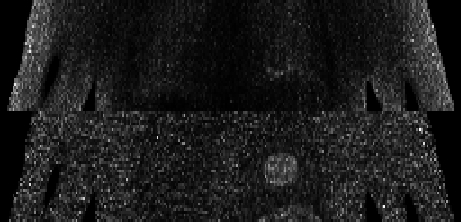
\includegraphics[scale=0.3]{figures/mcr.png}
    \caption{From top to bottom: MCR of the non-TOF data, MCR of the TOF data.}
    \label{fig:mcr}
\end{figure}

Following~\cite{McClelland2013}, we can write a motion model as a linear combination of surrogate signal (direct correspondence model). In the case of two surrogate signals, the following bivariate model can be used:
\begin{equation}
    \bm{M} = \phi(s_1,s_2)=\sum_{i=0}^{n}\sum_{j=0}^{n-i}\bm{A}_{i,j}s_1^i s_2^j
\end{equation}
where $s_1$ and $s_2$ are the surrogate signals and $\bm{A}_{i,j}$ a vector of polynomial coefficients (of order $n$). 
To estimate the motion models, NiftyRegResp was used using the sum of squared differences as objective function~\cite{NiftyRegResp}. The surrogate signal passed to NiftyRegResp consisted of both the displacement of the anterior-posterior and the  diaphragm movement from XCAT. For illustration, Figure~\ref{fig:mcr} shows the NAC motion-compensated reconstructions (MCR) obtained by NiftyRegResp after estimation of the motion models.

In order to evaluate the motion models generated, the estimated deformation fields were used to warp the ground truth PET volume, which was generated by XCAT at the mean position of the breathing cycle as discussed above. These warped images should be as close as possible to the original 6 input volumes generated by XCAT. The motion model calculated from the PET XCAT images was compared to the motion model calculated from nonTOF NAC reconstructions and the TOF NAC reconstruction.  

% The volumes created using the motion model calculated from the input data could be considered to be the ground truth estimated input volumes to which the volumes estimated from the motion models calculated from the nonTOF and TOF data could be compared.

\section{Results}
\begin{figure}
    \centering
    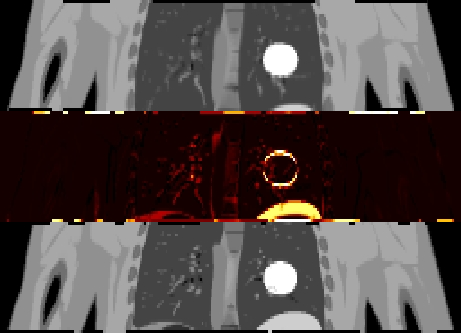
\includegraphics[scale=0.3]{figures/non_tof.png}
    \caption{From top to bottom: ground truth motion model applied to ground truth volume, differences between the two volumes, motion model estimated from the nonTOF data applied to ground truth volume. All volumes correspond to end-inhalation}
    \label{fig:non_tof}
\end{figure}

Figure~\ref{fig:non_tof} shows the difference between the ground truth and the nonTOF derived motion model at end-inhalation, as can be seen there is a great deal of variation between the two images when it comes to the motion of the lesion and liver. This is backed up by the mean squared error (MSE) between the two volumes, which is 97538.

\begin{figure}
    \centering
    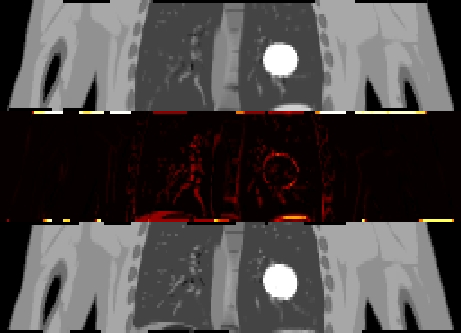
\includegraphics[scale=0.3]{figures/tof.png}
    \caption{From top to bottom: ground truth motion model applied to ground truth volume, differences between the two volumes, motion model estimated from the nonTOF data applied to ground truth volume. All volumes correspond to end-inhalation}
    \label{fig:tof}
\end{figure}

Figure~\ref{fig:tof} shows the difference between the ground truth and the TOF derived motion model at end-inhalation, when compared to figure~\ref{fig:non_tof} there is significantly less difference between the positions of the lesion and liver. This is again backed up by the MSE, especially when the MSE of the nonTOF data and the TOF data are compared. The MSE between the ground truth volume and the TOF volume is 62691 which is almost a third less than the MSE between the ground truth volume and the nonTOF volume, with an absolute difference of 34846.

\begin{figure}
    \centering
    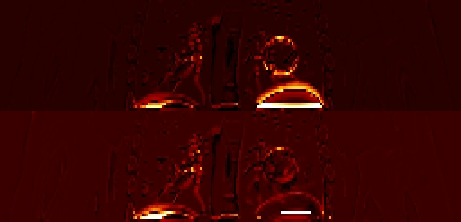
\includegraphics[scale=0.3]{figures/sum.png}
    \caption{From top to bottom: normalised differences between the ground truth and nonTOF volume, normalised differences between the ground truth and TOF volume. All volumes correspond to a sum over all gates.}
    \label{fig:sum}
\end{figure}

\begin{table}
    \centering
    \begin{tabular}{lll}
        \textbf{MSE}  & \textbf{nonTOF} & \textbf{TOF} \\
        \textbf{1}    & 115572          & 71557        \\
        \textbf{2}    & 49773           & 37059        \\
        \textbf{3}    & 97538           & 62691        \\
        \textbf{4}    & 73340           & 48010        \\
        \textbf{5}    & 64392           & 49269        \\
        \textbf{6}    & 115572          & 71557        \\
        \textbf{Mean} & 86031           & 56691       
    \end{tabular}
    \caption{This table shows a comparison of the MSE for both the nonTOF data and the TOF data over all gates plus the mean MSE over all gates.}
    \label{tab:mse}
\end{table}

Figure~\ref{fig:sum} shows the normalised difference between the ground truth and the nonTOF derived motion model and the ground truth and the TOF derived motion model summed over all gates. As can be seen the assertion that the difference between the position of the lesion and liver is greater for the nonTOF data then the TOF holds true over all gates. This is supported when the MSE over all gates is compared as can be seen in table~\ref{tab:mse}, the difference between the mean MSE of the nonTOF data and the TOF data is 29341.

% needed in second column of first page if using \IEEEpubid
%\IEEEpubidadjcol

% An example of a floating figure using the graphicx package.
% Note that \label must occur AFTER (or within) \caption.
% For figures, \caption should occur after the \includegraphics.
% Note that IEEEtran v1.7 and later has special internal code that
% is designed to preserve the operation of \label within \caption
% even when the captionsoff option is in effect. However, because
% of issues like this, it may be the safest practice to put all your
% \label just after \caption rather than within \caption{}.
%
% Reminder: the "draftcls" or "draftclsnofoot", not "draft", class
% option should be used if it is desired that the figures are to be
% displayed while in draft mode.
%
%\begin{figure}[!t]
%\centering
%\includegraphics[width=2.5in]{myfigure}
% where an .eps filename suffix will be assumed under latex, 
% and a .pdf suffix will be assumed for pdflatex; or what has been declared
% via \DeclareGraphicsExtensions.
%\caption{Simulation results for the network.}
%\label{fig_sim}
%\end{figure}

% An example of a double column floating figure using two subfigures.
% (The subfig.sty package must be loaded for this to work.)
% The subfigure \label commands are set within each subfloat command,
% and the \label for the overall figure must come after \caption.
% \hfil is used as a separator to get equal spacing.
% Watch out that the combined width of all the subfigures on a 
% line do not exceed the text width or a line break will occur.
%
%\begin{figure*}[!t]
%\centering
%\subfloat[Case I]{\includegraphics[width=2.5in]{box}%
%\label{fig_first_case}}
%\hfil
%\subfloat[Case II]{\includegraphics[width=2.5in]{box}%
%\label{fig_second_case}}
%\caption{Simulation results for the network.}
%\label{fig_sim}
%\end{figure*}
%
% Note that often IEEE papers with subfigures do not employ subfigure
% captions (using the optional argument to \subfloat[]), but instead will
% reference/describe all of them (a), (b), etc., within the main caption.
% Be aware that for subfig.sty to generate the (a), (b), etc., subfigure
% labels, the optional argument to \subfloat must be present. If a
% subcaption is not desired, just leave its contents blank,
% e.g., \subfloat[].

% An example of a floating table. Note that, for IEEE style tables, the
% \caption command should come BEFORE the table and, given that table
% captions serve much like titles, are usually capitalized except for words
% such as a, an, and, as, at, but, by, for, in, nor, of, on, or, the, to
% and up, which are usually not capitalized unless they are the first or
% last word of the caption. Table text will default to \footnotesize as
% the IEEE normally uses this smaller font for tables.
% The \label must come after \caption as always.
%
%\begin{table}[!t]
%% increase table row spacing, adjust to taste
%\renewcommand{\arraystretch}{1.3}
% if using array.sty, it might be a good idea to tweak the value of
% \extrarowheight as needed to properly center the text within the cells
%\caption{An Example of a Table}
%\label{table_example}
%\centering
%% Some packages, such as MDW tools, offer better commands for making tables
%% than the plain LaTeX2e tabular which is used here.
%\begin{tabular}{|c||c|}
%\hline
%One & Two\\
%\hline
%Three & Four\\
%\hline
%\end{tabular}
%\end{table}

\section{Conclusion}
In conclusion, because there is such a drastic improvement in the images, both visually and when comparing the MSE, it is likely that the TOF derived motion model more accurately estimates the ground truth motion than the nonTOF derived motion model. This is especially true when it comes to lesions which fall close to the lung/liver boundary as the greatest improvement can be seen there.

In addition because it is the motion of the heavily attenuated internal organs that would be most useful (in an iterative joint reconstruction motion correction algorithm~\cite{Bousse2016a} being started by this initial estimation) to warp the static attenuation map to each gate, then because the TOF derived motion model estimates this motion better, than the nonTOF derived motion model, it would be superior in this use case.

However, a large disadvantage of the TOF reconstruction is that it greatly increases the computational time of both the reconstruction and the calculation of the motion model.

Future work will involve taking the concept of the NAC TOF derived motion model and applying it as the starting point for an iterative joint reconstruction motion correction algorithm, as discussed above.

% Can use something like this to put references on a page
% by themselves when using endfloat and the captionsoff option.
\ifCLASSOPTIONcaptionsoff
  \newpage
\fi

% trigger a \newpage just before the given reference
% number - used to balance the columns on the last page
% adjust value as needed - may need to be readjusted if
% the document is modified later
%\IEEEtriggeratref{8}
% The "triggered" command can be changed if desired:
%\IEEEtriggercmd{\enlargethispage{-5in}}

% references section

% can use a bibliography generated by BibTeX as a .bbl file
% BibTeX documentation can be easily obtained at:
% http://mirror.ctan.org/biblio/bibtex/contrib/doc/
% The IEEEtran BibTeX style support page is at:
% http://www.michaelshell.org/tex/ieeetran/bibtex/
%\bibliographystyle{IEEEtran}
% argument is your BibTeX string definitions and bibliography database(s)
%\bibliography{IEEEabrv,../bib/paper}
%
% <OR> manually copy in the resultant .bbl file
% set second argument of \begin to the number of references
% (used to reserve space for the reference number labels box)
% \begin{thebibliography}{1}

% \bibitem{IEEEhowto:kopka}
% H.~Kopka and P.~W. Daly, \emph{A Guide to \LaTeX}, 3rd~ed.\hskip 1em plus
%   0.5em minus 0.4em\relax Harlow, England: Addison-Wesley, 1999.

% \end{thebibliography}

%\bibliographystyle{IEEEtran}
%\bibliography{./bibtex/bib/Biblio}

\AtNextBibliography{\small}
\printbibliography

%\vfill

% Can be used to pull up biographies so that the bottom of the last one
% is flush with the other column.
%\enlargethispage{-5in}

% that's all folks
\end{document}
